\newcommand{\norm}[1]{\parallel #1 \parallel_2}
%%\subsection{B--Spline}
%\begin{frame}{Least sqare fitting problem}
%\begin{overlayarea}{\textwidth}{.15 \textheight}
%\begin{enumerate}
%\item Coarse approximating quad from Dual Contouring
%\item<2-> Projection of datapoint onto plane
%\item<3-> Task: Find corresponding parameters for B-Spline surface $\left[u,v\right] \in \left[0,1\right]^2$
%\end{enumerate}
%\end{overlayarea}
%\begin{overlayarea}{\textwidth}{.85 \textheight}
%\begin{columns}
%\column{.35\textwidth}
%
%\begin{overlayarea}{\textwidth}{\textheight}
%\begin{figure}
%\only<1-4>{
%\tdplotsetmaincoords{60}{110}
%\begin{tikzpicture}[scale = 1.5,tdplot_main_coords]
%\coordinate (O) at (-1,-1,0);
%\coordinate[dot] (A) at (0,0,0);
%\coordinate[dot] (B) at (1,0,0);
%\coordinate[dot] (C) at (1.2,1.5,0);
%\coordinate[dot] (D) at (0,1,0);
%\only<3->{
%\coordinate[dot] (E) at (1.4,2.0,-0.5);
%\coordinate[dot] (F) at (0,1.7,-0.8);
%\draw[thick] (D) -- (F) -- (E) -- (C);}
%
%\coordinate (P1) at (.5,.4,1);
%\coordinate (P2) at (1,1,1);
%\coordinate (P3) at (0.2,0.2,2);
%\coordinate (P4) at (0.1,1.3,1);
%
%
%\coordinate (Q1) at (.5,.4,0);
%\coordinate (Q2) at (1,1,0);
%\coordinate (Q3) at (0.2,0.2,0);
%\coordinate (Q4) at (0.1,0.9,0);
%
%
%
%\draw[thick,->] (O) -- ($(O)+(.5,0,0)$) node[anchor=north east]{$x$};
%\draw[thick,->] (O) -- ($(O)+(0,.5,0)$) node[anchor=north west]{$y$};
%\draw[thick,->] (O) -- ($(O)+(0,0,.5)$) node[anchor=south]{$z$};
%
%\draw[thick] (A) -- (B) -- (C) -- (D) -- (A);
%
%\only<2-4>{
%\draw (P1) node[thick,cross,red,label = {$P_1$}] {};
%\draw[red,dashed] (P1) -- (Q1);
%\draw (Q1) node[thick,cross,red] {};
%\draw (P2) node[thick,cross,red,label = {$P_2$}] {};
%\draw[red,dashed] (P2) -- (Q2);
%\draw (Q2) node[thick,cross,red] {};
%\draw (P3) node[thick,cross,red,label = {$P_3$}] {};
%\draw[red,dashed] (P3) -- (Q3);
%\draw (Q3) node[thick,cross,red] {};
%}
%\only<3->{
%\draw (P4) node[thick,cross,red,label = {$P_4$}] {};
%\draw[red,dashed] (P4) -- (Q4);
%\draw (Q4) node[thick,cross,red] {};
%
%}
%\draw (A) node[label = left:{$A$}]{};
%\draw (B) node[label = left:{$B$}]{};
%\draw (C) node[label = right:{$C$}]{};
%\draw (D) node[label = right:{$D$}]{};
%\only<3->{
%\draw (E) node[label = right:{$E$}]{};
%\draw (F) node[label = right:{$F$}]{};}
%\only<4>{
%\coordinate[dot] (A2) at (0,0,1);
%\coordinate[dot] (B2) at (1,0,1);
%\coordinate[dot] (D2) at (0.,1.5,0.9);
%\coordinate[dot] (C2) at (1,1.9,1);
%\draw [dashed] (A2)--(D2) --(C2) -- (B2) -- (A2);
%%\draw (C2) node[label = right:{$C'$}]{};
%%\draw (D2) node[label = right:{$D'$}]{};
%%\draw (A2) node[label = right:{$A'$}]{};
%%\draw (B2) node[label = right:{$B'$}]{};
%
%}
%\end{tikzpicture}
%}
%\end{figure}
%\end{overlayarea}
%
%\column{.5\textwidth}
%\begin{overlayarea}{\textwidth}{\textheight}
%\only<3->{
%\begin{block}{Problem:}
%\begin{itemize}
%\item Fit B-Spline surface, that is C0 and C1 continuous on the borders
%\end{itemize}
%\end{block}
%
%\begin{block}{Solution:}
%\begin{enumerate}
%\item Method: Peter's scheme
%\item Solve (coupled) global system of equations
%\end{enumerate}
%\end{block}
%
%}
%\end{overlayarea}
%\end{columns}
%\end{overlayarea}
%\end{frame}

\begin{frame}{Peters' Scheme revisited}
%\begin{block}{Peters' scheme:}
%Given the control mesh $M_{x}$
%\begin{enumerate}
%\item Refine the \textit{control mesh} 2 times using Doo-Sabin refinement
%\item Construct a tensor product Bezier patches (biquadratic or bicubic) centred on the each vertex of the refined \textit{control mesh}
%\end{enumerate}
%\end{block}
%\begin{overlayarea}{\textwidth}{.1\textheight}
%	\only<1>{Control mesh}
%	\only<2>{Refined control mesh}
%	\only<3>{Bezier control points}
%	\only<4>{B-Spline patch}
%	\only<5>{Peters' surface}
%\end{overlayarea}
\begin{overlayarea}{\textwidth}{.9\textheight}
    \begin{center}
		\begin{tikzpicture} 
        
        \node at (0,3.5)[inner sep=0pt, scale = 0.5](N1)
                {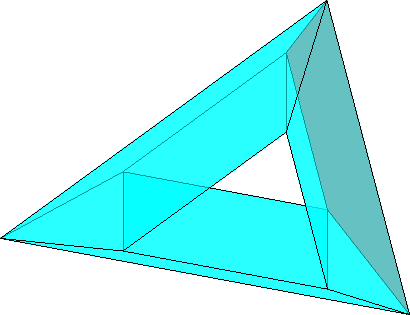
\includegraphics[width=5cm]{Pictures/NURBS/tikz/control_mesh.pdf}};
        
        \node at (3.5,3.5) [inner sep=0pt, scale = 0.5](N2)
        			{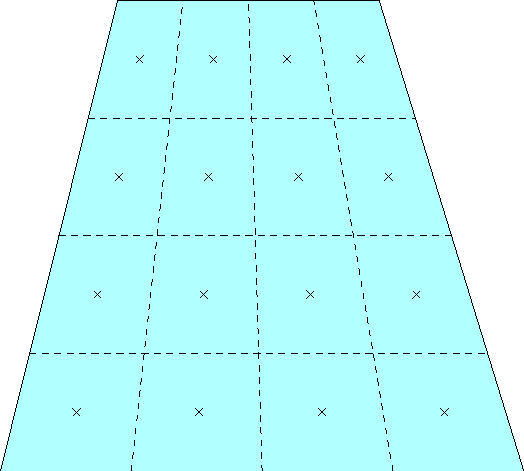
\includegraphics[width=5cm]{Pictures/NURBS/tikz/patch_points.pdf}};
        			                  
        \draw[thick,->] (N1) -- (N2);
        
        
        \node at (7,2)[inner sep=0pt, scale = 0.5](N3)
                  {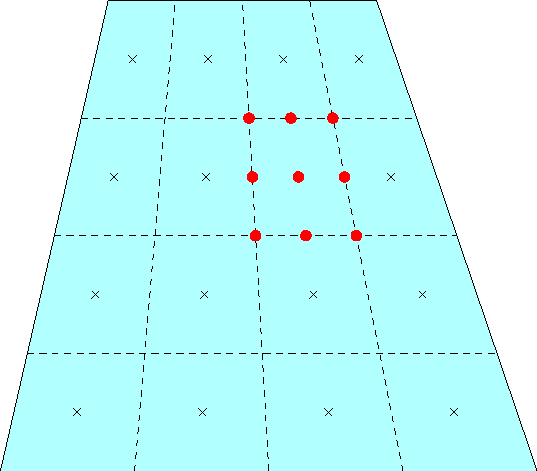
\includegraphics[width=5cm]{Pictures/NURBS/tikz/bezier_points.pdf}};
        \draw[thick,->] (N2) -- (N3);
        
        
        \node at (3.5, 0)[inner sep=0pt, scale = 0.5](N4)
                {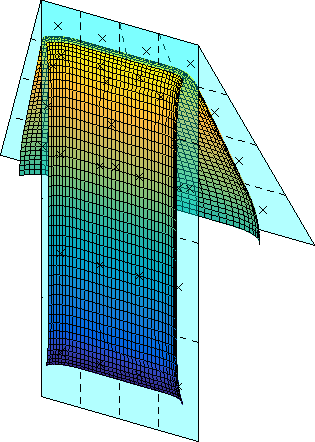
\includegraphics[width=5cm]{Pictures/NURBS/tikz/bspline_patches.pdf}};
        \draw[thick,->] (N3) -- (N4);
        
        
        \node at (0, 0)[inner sep=0pt, scale = 0.5](N5)
                 {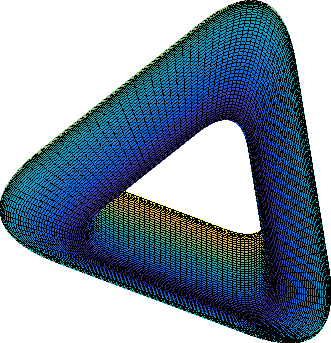
\includegraphics{Pictures/NURBS/tikz/torus_peters.pdf}};
        \draw[thick,->] (N4) -- (N5);
        
        \end{tikzpicture}
	\end{center}
\end{overlayarea}
%\textbf{{\color{red} According to Peters obtained surface is $G^{1}$ smooth}}
\end{frame}

\begin{frame}{Fitting Problem: Peters’ Scheme\textsuperscript{3}}
\vspace{-0.5cm}
\only<1>{
\begin{minipage}[t]{0.4\linewidth}
\begin{figure}
	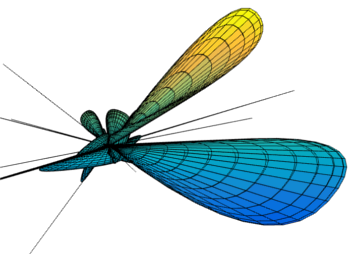
\includegraphics[width=.88\textwidth]{Pictures/NURBS/mosquito_surface}
\end{figure}
\end{minipage}%
\hfill%
\begin{minipage}[t]{0.55\linewidth}
%\begin{block}{}
\vspace{0.27cm}
\begin{equation*}
||D - C(u, v) \ P||^2  \rightarrow min %\sum_{i=1}^{N}\norm{P_{i} - y_{i}V_{x}}^{2} \rightarrow min$$
\end{equation*}
%\end{block}
\end{minipage}}

\only<2>{
\begin{minipage}[t]{0.4\linewidth}
\begin{figure}
	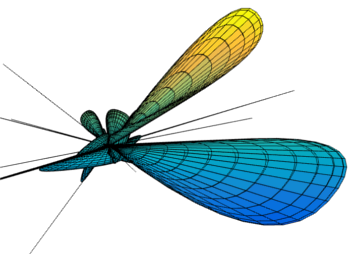
\includegraphics[width=.88\textwidth]{Pictures/NURBS/mosquito_surface}
\end{figure}
\end{minipage}%
\hfill%
\begin{minipage}[t]{0.55\linewidth}
%\begin{block}{}
\begin{equation*}
||D - C(u, v) \ P||^2 + \textcolor{red}{\lambda ||0-C^{fair}P||}  \rightarrow min %\sum_{i=1}^{N}\norm{P_{i} - y_{i}V_{x}}^{2} \rightarrow min
\end{equation*}
%\end{block}
\end{minipage}}
\vspace{0.2cm}
\only<1>{
\begin{minipage}[t]{0.4\linewidth}
\begin{figure}
	
\includegraphics[width=.88\textwidth]{Pictures/NURBS/ToCover}
\end{figure}
\end{minipage}%
\hfill%
\begin{minipage}[t]{0.55\linewidth}
\begin{block}{Notation}
$D$ - Data  points object to surface fitting\\
$C(u,v)$ - Control Point Matrix \\
$P$ - B-Spline Control Points \\
\end{block}
\end{minipage}}

\only<2>{
\begin{minipage}[t]{0.4\linewidth}
\begin{figure}
	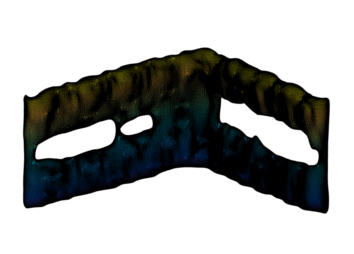
\includegraphics[width=.88\textwidth]{Pictures/NURBS/MosquitoNo}
\end{figure}
\end{minipage}%
\hfill%
\begin{minipage}[t]{0.55\linewidth}
\begin{block}{Notation}
$D$ - Data  points object to surface fitting\\
$C(u,v)$ - Control Point Matrix \\
$P$ - B-Spline Control Points \\
\color{red}{$C^{fair}$ - Fairness coefficients}
\end{block}
\end{minipage}}

\end{frame}
